\clearpage
\appendix

% AH-135143

\section{Results on Additional Model Pairs}
\label{appendix:additional}

We conducted experiments on additional model pairs, summarized in Table~\ref{tab:avg6}, which highlights the cumulative performance gains across tasks for six different model pairs. The model pairs include: (1) merging LLaVA-OneVision \cite{llava-onevison} into Qwen2-VL \cite{qwen2-vl} (Table~\ref{tab:llava2qwen}), (2) merging LLaVA-v1.5 \cite{llava1.5} into CogVLM \cite{cogvlm} (Table~\ref{tab:cogvlm}), (3) merging mPLUG-Owl2 into LLaVA-v1.5, (4) merging LLaVA-v1.5 into mPLUG-Owl2 \cite{mplugowl2} (Table~\ref{tab:llava2mplug}), (5) merging CogVLM into mPLUG-Owl2 (Table~\ref{tab:cog2mplug}) and (6) merging mPLUG-Owl2 into CogVLM (Table~\ref{tab:mplug2cog}).
% \ours demonstrates strong effectiveness by achieving the highest overall performance gain and consistently ranking among the top two for improvements on all tasks. 
The performance gain for each task is computed as the difference between the performance of our method (or baselines) and the average performance of the two original models, with positive values indicating an improvement.
In Table~\ref{tab:avg6}, the SUM column presents the total performance gains across all tasks, where \ours outperforms all baselines, achieving +91.92 performance gain, and consistently ranks among the top two in performance gains across all benchmarks.
It is noteworthy that on GQA \cite{gqa} and VizWiz \cite{vizwiz} benchmarks in Table~\ref{tab:llava2mplug} and Table~\ref{tab:cog2mplug}, all model merging methods experience a performance drop. We attribute this decline to the significant performance gap between the original models on these benchmarks. In these scenarios, \ours demonstrates the smallest performance decrease among them.
In Table~\ref{tab:llava2mplug}, Table~\ref{tab:cog2mplug} and Table~\ref{tab:mplug2cog}, \ours obtains the second best result in the sum of all benchmarks, with a small gap compared to the best baseline. 

To investigate the effect of altering base models on performances, we analyze experiments on merging the same model pair with different base models. For the model pair of mPLUG-OWl2 and CogVLM, results in Table~\ref{tab:cog2mplug} use mPLUG-Owl2 as the base model, and results in Table~\ref{tab:mplug2cog} use CogVLM as the base model.
On benchmarks where the original models exhibit a significant performance gap, such as OCRBench \cite{ocrbench} and TextVQA \cite{textvqa}, model merging methods, including \ours, achieve only marginal performance improvements. In contrast, on benchmarks where the original models have comparable performance, \ours consistently enhances the base model’s performance (with the exception of GQA \cite{gqa} for the mPLUG-Owl2 architecture), irrespective of the choice of base model.
Notably, even when merging a weaker model into a stronger one for a specific task, \ours can sometimes boost the stronger model's performance. For instance, this effect is observed on SEEDBench \cite{seedbench}, OKVQA \cite{okvqa}, and GQA \cite{gqa} in Table~\ref{tab:mplug2cog}. These results highlight that our model merging technique can further optimize the performance of a strong model, even when another model demonstrates weaker performance on the same task.

Additionally, to demonstrate the effectiveness of our method on larger models, we conducted experiments on Cambrian and Yi-VL with 34B language model size. Table~\ref{tab:larger} shows that \textbf{\ours also merges the abilities in larger MLLMs effectively}.

\begin{table}[!ht]
    \centering\small
    \begin{tabular}{lll}
    \hline
        Model & $\mathrm{OCRBench}$ & $\mathrm{MME}$  \\ \hline
        Cambrian\footnotesize(base) & 58.70 & 72.50 \\ 
        Yi-VL & 29.70 & 73.65\\ 
        AVG & 44.20 & 73.08  \\        
        AdaMMS & \textbf{59.20} & \textbf{74.07}  \\ \hline
    \end{tabular}
    \caption{Results on merging Yi-VL into Cambrian.}
    \label{tab:larger}
\end{table}


\section{Implementation Details of \ours}
\label{appendix:impl}

The implementation details of \ours are as follows:

\noindent\textbf{Mapping} \  In this step, we identify parameters in the language models that account for additional weights. For CogVLM \cite{cogvlm}, all weights within the visual experts in the attention mechanism (including the QKV matrix and the FFN of the visual expert) are treated as additional weights. For mPLUG-Owl2 \cite{mplugowl2}, vision representation weights within the Modality-Adaptive Modules (such as the decoupled vision layer-norm and KV matrix) are considered additional weights. For different vision encoders, the vision encoder weights of the base model are retained as the final weights after merging, regardless of the vision encoder in the other model.

\noindent\textbf{Merging} \  During this step, we first merge the weights in the language model of the base model. If the weights are not classified as additional weights in the Mapping step, they are merged using linear interpolation or other baseline merging techniques. For weights categorized as additional weights, we check whether the other model has duplicated the same weights. Based on this, we (1) merge the weights if duplicates exist, or (2) retain the original weights in the base model if no duplicates are found.

\noindent\textbf{Searching} \  In the final step, we randomly select a subset of 100 test inputs to determine the optimal $\alpha$. For each $\alpha$ candidate, we generate model responses for the selected inputs. To select the best $\alpha$, we apply the Exact Match metric for the total difference score: for each input, if the merged model's response with a given $\alpha$ matches the response with adjacent $\alpha$ values, the difference score is 0; otherwise, it is 1. The total difference score is the sum of scores across all inputs in the subset. The $\alpha$ with the lowest total difference score is selected as the final choice. Note that the small subset of 100 inputs is randomly sampled using the method in LMMs-Eval framework \cite{lmms-eval}. We have repeated the sampling process to ensure that the randomness in sampling does not affect the performance of our method.

\section{Evaluation Details}
\label{appendix:eval}
% frameworks and prompts

We utilize LMMs-Eval \cite{lmms-eval} and VLMEvalKit \cite{vlmevalkit}, two open-source evaluation frameworks for MLLMs, to assess our models. Specifically, for evaluating MMMU \cite{mmmu}, MME \cite{mme}, SEEDBench \cite{seedbench}, OCRBench \cite{ocrbench}, and TextVQA \cite{textvqa} within the Qwen2-VL \cite{qwen2-vl} architecture, we use the VLMEvalKit framework, while LMMs-Eval is employed for the others. To ensure consistency with the reported results for LLaVA and mPLUG-Owl2 on OK-VQA \cite{okvqa}, we adapted the prompt template in the evaluation framework, as detailed in Table~\ref{tab:prompt}. Other prompt templates remains the same in the evaluation frameworks.

\section{Comparing Supervised and Unsupervised}
\label{appendix:unsupervised}

We compared \ours with baseline merging methods with supervised hyper-parameter selection. Due to the absence of separate test sets, we trained the supervised baseline on either a subset or the entirety of the evaluation set. \textbf{This implies that the supervised baseline was in a more favorable position compared to our method, as our method does not have access to the groudtruth labels.} Table~\ref{tab:supervised} shows that \ours still outperforms it, indicating the superiority of our unsupervised method.

% \section{Results on Merging Language Models}
% \label{appendix:llm}

% We conduct experiments on merging Qwen2.5-Math and Qwen2.5-Coder, which is evaluated on GSM8K and HumanEval benchmarks. Result in Table~\ref{tab:llm} shows that only \ours is still effective in merging language models. Baselines use the same hyper-parameters as the main experiments but perform poorly, highlighting the heightened sensitivity of LLM merging to hyper-parameter tuning.

\section{Intermediate Results in Searching}
\label{appendix:searching}
%diff和acc的趋势图

%alpha具体的表格
We present an example of the intermediate results during the selection of $\alpha$. As shown in Figure~\ref{tab:inter_alpha}, \ours effectively identifies a near-optimal $\alpha$, achieving performance close to the best possible outcome. Specifically, our unsupervised hyper-parameter selection method successfully chooses the optimal $\alpha$ candidate in half of the benchmarks and maintains a deviation of no more than 0.2 from the best $\alpha$ in the remaining cases.

Figure~\ref{fig:consistency_acc4} illustrates the relationship between model performance and generation consistency across MMMU, MME, SeedBench, and OCRBench when merging LLaVA-OneVision into Qwen2-VL. The observed trends validate our approach in the search step, where model performance is approximated using generation consistency without relying on labeled data. Notably, for these tasks, the $\alpha$ selected by our method corresponding to the highest generation consistency deviates from the $\alpha$ achieving the best performance by no more than 0.1, showing that our hyper-parameter selection method achieves near-optimal performance.

\begin{table}[h]
   
     \resizebox{0.478\textwidth}{!}{%
    \begin{tabular}{ccc}
    \hline
        Framework & Base Model & Prompt   \\ \hline
        \multirow{2}{*}{LMMs-Eval} & LLaVA &  \multirow{2}{*}{Answer the question using a single word or phrase.} \\
         & mPLUG-Owl2 &  \\ \hline
          
    \end{tabular}
    }
    \caption{Altered prompt for evaluation on OK-VQA.}
    \label{tab:prompt}
\end{table}

\section{Supplementary Proof}
\label{appendix:proof}

We provide the following proof as the theoretical justification for relationship between generation consistency correlates and model performance.

\noindent\textit{Proof.} Using the notation in Section~\ref{searching}, for an arbitrary task $t_i$, let $S_{t_i}(\alpha)$ be the ratio of correct answer at position $\alpha$, and $D_{t_i}(\alpha; \alpha^-)$ be the ratio of the difference in generated responses between position $\alpha$ and its adjacent candidate $\alpha^-$.
Since the difference in $S_{t_i}(\alpha)$ is only influenced  by the subset of generated responses where the correctness status changes (i.e., transitions between correct and incorrect), we have $|S_{t_i}(\alpha)-S_{t_i}(\alpha^-)| \leq D_{t_i}(\alpha; \alpha^-)$. For the same reason with $\alpha^+$, we can prove  $|S_{t_i}(\alpha)-S_{t_i}(\alpha^-)| + |S_{t_i}(\alpha)-S_{t_i}(\alpha^+)| \leq 2D_{t_i}(\alpha; \alpha^-, \alpha^+)$.
Therefore, a higher generation consistency with small $D_{t_i}(\alpha; \alpha^-, \alpha^+)$ implies a higher model performance $S_{t_i}(\alpha)$, due to its convexity.

\section{Experimental Results in Granularity for \texorpdfstring{$\alpha$}{alpha}}
\label{appendix:granularity}

Figure~\ref{fig:step_size} presents the result of \ours at different granularities of $\alpha$. The point in stars indicates the best $\alpha$ by our unsupervised parameter selection method. The result shows that these granualities in $\{0.02, 0.05, 0.10\}$ behave similarly in terms of the final performance, indicating the robustness of \ours. Therefore, in practice we choose a larger $\alpha$ so that we have fewer $\alpha$ candidates, which reduces the computation cost.

% \twocolumn[{%
%     \renewcommand\twocolumn[1][]{#1} % 临时打破双栏布局
\begin{table*}[t]
    \centering
    
     \resizebox{\textwidth}{!}{
    \begin{tabular}{lllllllllll}
    \hline
        Model & $\mathrm{MMMU_{val}}$ & $\mathrm{MME_{sum}}$ & $\mathrm{SeedBench_{all}}$ & $\mathrm{OCRBench}$ & $\mathrm{TextVQA_{val}}$ & $\mathrm{OKVQA}$ & $\mathrm{GQA}$ & $\mathrm{VizWiz_{val}}$ & $\mathrm{Sum}$ & $\mathrm{Diff}$  \\ \hline
        AdaMMS & 34.90  & 69.09  & 64.12  & 55.70  & 76.90  & 61.11  & 60.12  & 37.27  & 459.21  & +31.23 \\ 
        Ties-Merging  & 34.00  & 57.29  & 38.97  & 55.00  & 59.73  & 40.31  & 51.97  & 24.36  & 361.63  & -66.35 \\ 
        Ties-Merging (supervised with 100 eval. samples) & 37.20  & 57.29  & 63.12  & 55.90  & 76.50  & 61.45  & 55.81  & 37.98  & 445.25  & +17.27 \\ 
        Ties-Merging (supervised with all eval. data) & 37.20  & 63.96  & 65.43  & 55.90  & 76.55  & 61.45  & 57.99  & 38.21  & 456.69  & +28.71 \\ 
        \hline
        
\end{tabular}
    }
    
    % \vspace{0.05cm}
    
    \captionof{table}{ \ours and Ties-Merging with \textit{supervised} hyper-parameter selection via validation set.}

    % \vspace{0.05cm}
    
    \label{tab:supervised}
    % \centering
    % \resizebox{\textwidth}{!}{
    % \begin{tabular}{lccccccccc}
    %     \hline
    %     Model        & Qwen2.5-Math(base) & Qwen2.5-Coder & AVG & Task Arithmetic & Ties-Merging & DARE-Linear & DARE-Ties & MetaGPT & AdaMMS \\ \hline
    %     GSM8K        & 84.23        & 69.45   & 76.84  & 40.94  & 0.00     & 0.00      & 0.00    & 54.81  & 80.21  \\ 
    %     HumanEval    & 32.93     & 80.49    & 56.71  & 0.00      & 0.00    & 0.00     & 0.00   & 4.88     & 40.85  \\ \hline
    % \end{tabular}}

    % \vspace{0.05cm}
    
    % \captionof{table}{ \footnotesize  Results on merging Qwen2.5-Coder with Qwen2.5-Math.}
    % \vspace{0.15cm}
    % \label{tab:llm}

% }]
\end{table*}

\begin{figure*}
    \centering
   
    \begin{subfigure}[b]{0.43\textwidth}
        \centering
        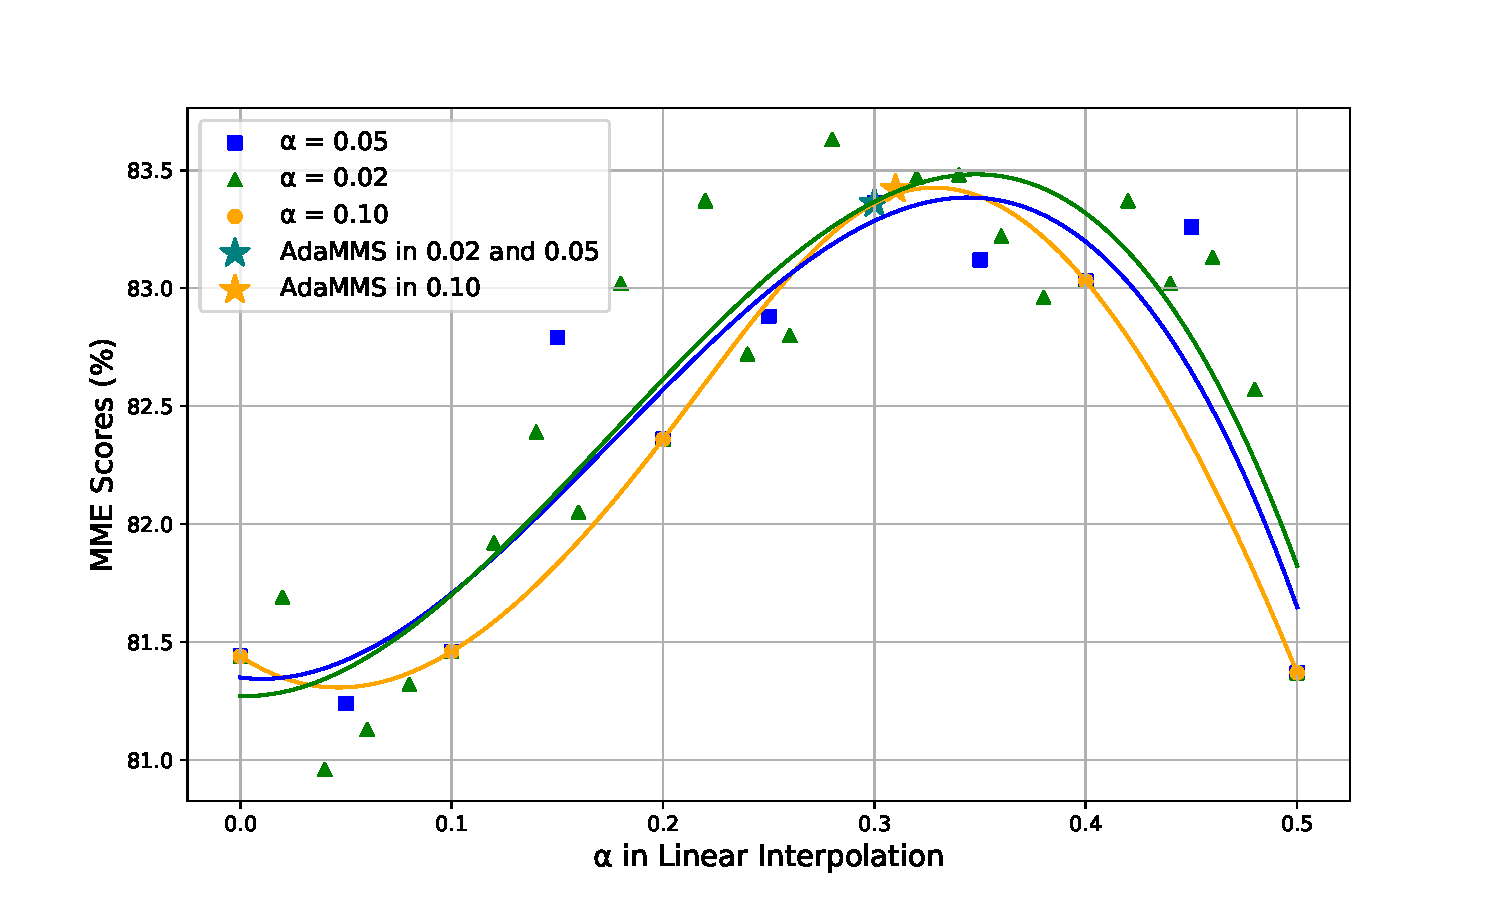
\includegraphics[width=\textwidth, bb=0 0 720 432]{figure/mme_values_plot_new.pdf}
        % \caption{图2的说明}
    \end{subfigure}
    \begin{subfigure}[b]{0.43\textwidth}
        \centering
        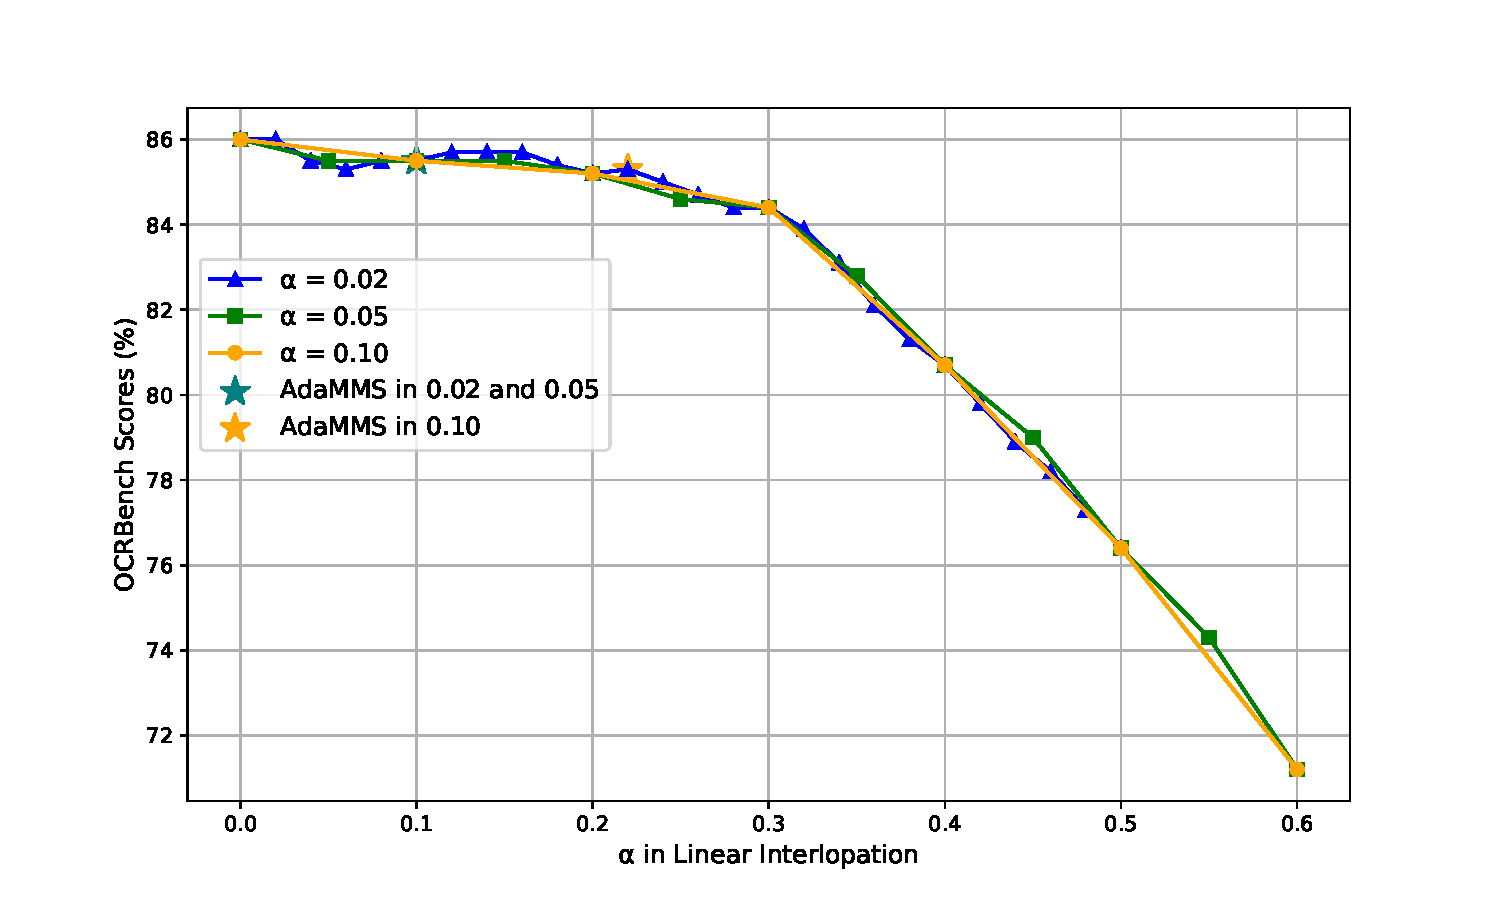
\includegraphics[width=\textwidth, bb=0 0 720 432]{figure/ocr_values_plot_new.pdf}
        % \caption{caption}
    \end{subfigure}
    \caption{Results on linear interpolation at different granularities of $\alpha$ when merging LLaVA-OneVison-7B into Qwen2-VL-7B-7B. (Left: MME, Right: OCRBench)}
    \label{fig:step_size}
\end{figure*}


\begin{figure*}[h]
    \centering
    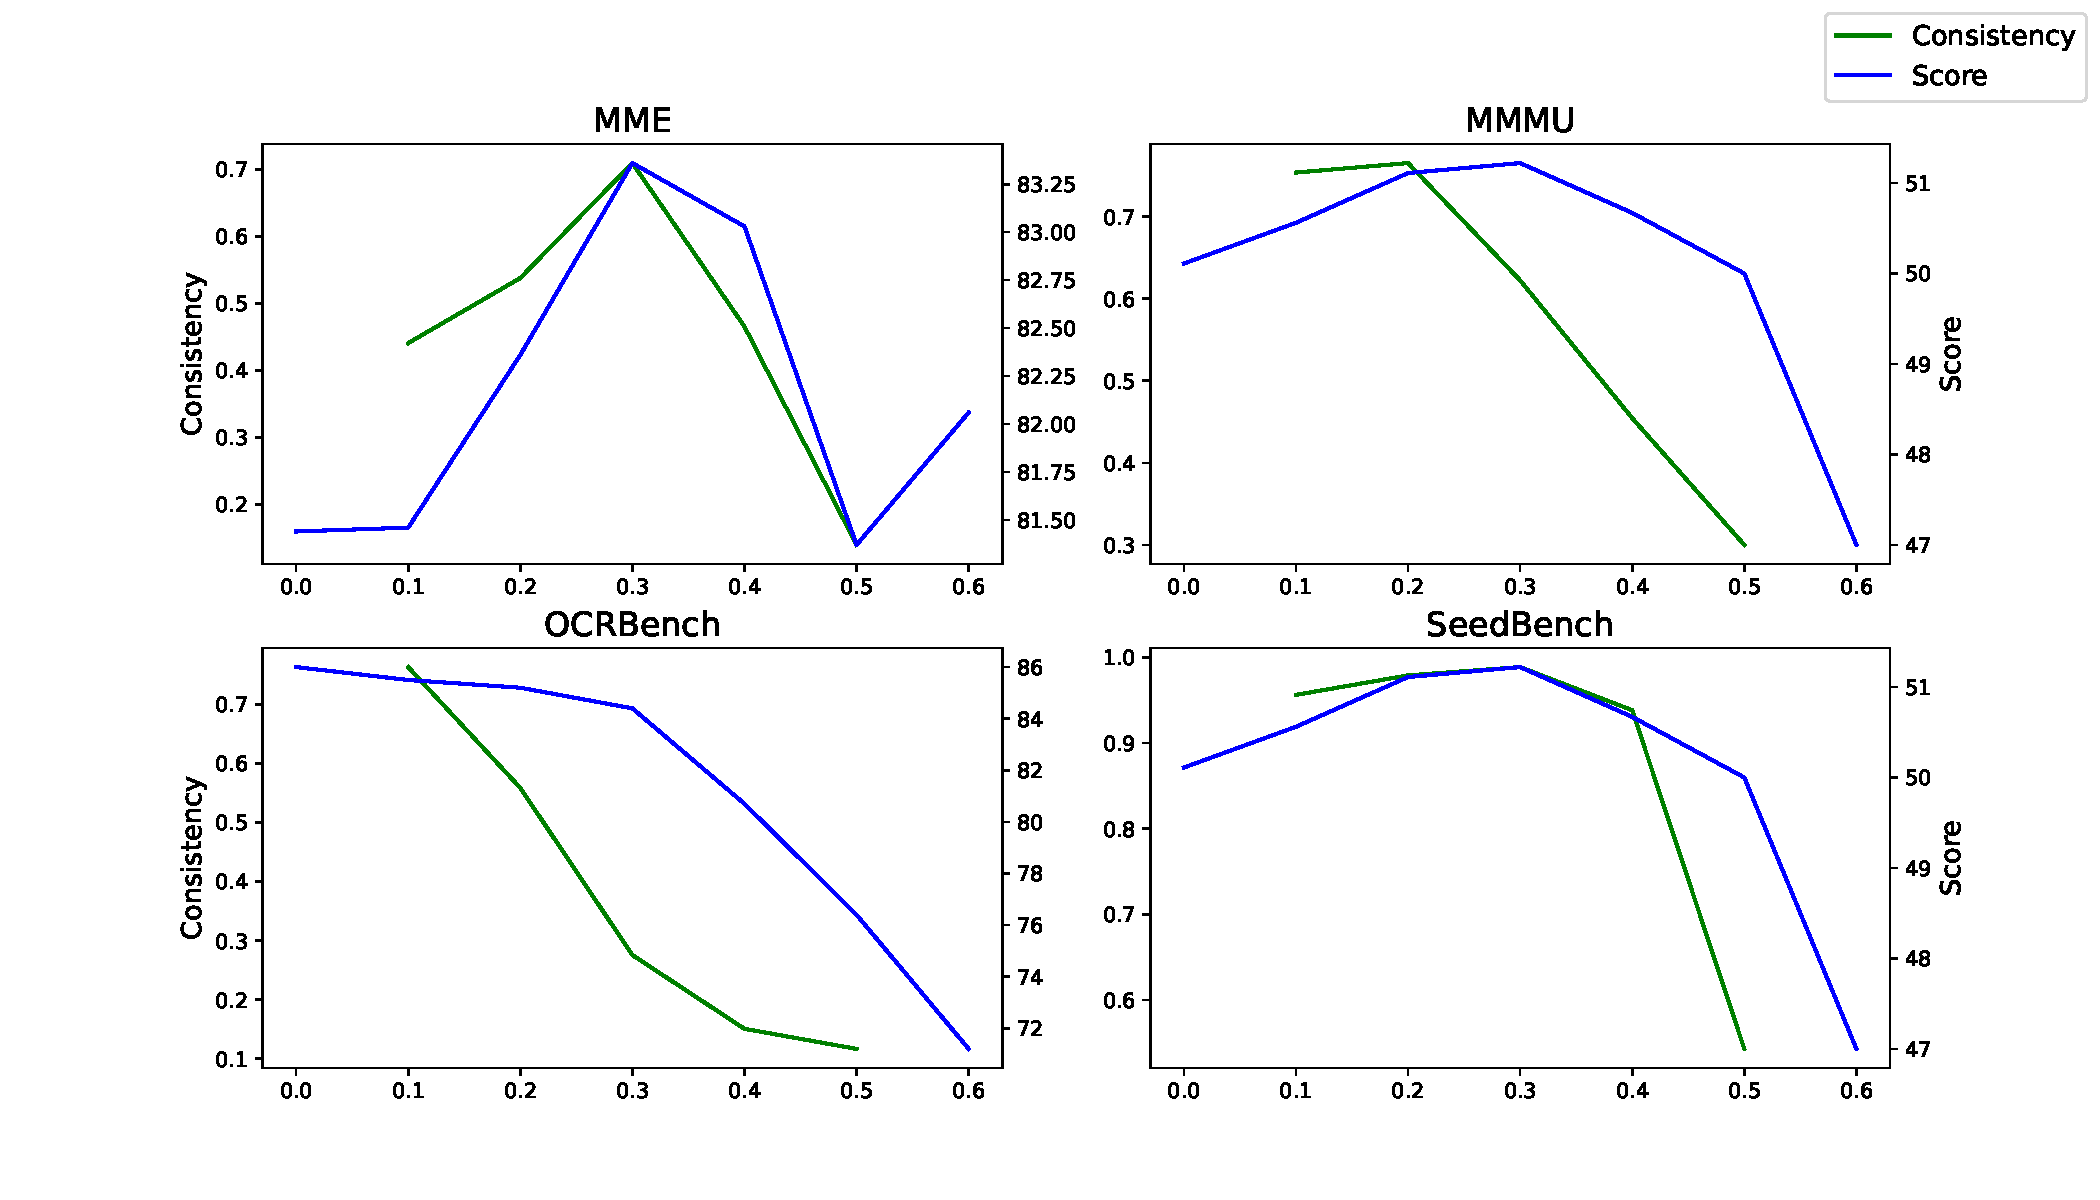
\includegraphics[width=\linewidth, bb=0 0 1007 576]{figure/consistency_acc4.pdf}
    \caption{Generation consistency and model performance (score) for MME, MMMU, OCRBench and SeedBench when merging LLaVA-OneVision-7B into Qwen2-VL-7B. Generation consistency is calculated as the reciprocal of the sum of different responses from models with adjacent $\alpha$ candidates. The horizontal axis is the $\alpha$ of the linear interpolation.}
    \label{fig:consistency_acc4}
\end{figure*}

% \section{Qualitative Results}
% \label{appendix:example}

% Figure X shows the qualitative results of \ours with examples on Y benchmark.


% \begin{table*}[!ht]
    \centering
       \resizebox{\textwidth}{!}{%      
    \begin{tabular}{lcccccccccc}
    \toprule
        \textbf{Model} & $\mathrm{MMMU_{val}}$ &  $\mathrm{MME_{sum}}$ &  $\mathrm{SeedBench_{all}}$ & $\mathrm{OCRBench}$  &  $\mathrm{TextVQA_{val}}$  & $\mathrm{OKVQA}$ & $\mathrm{GQA}$  &  $\mathrm{VizWiz_{val}}$ & $\mathrm{SUM}$ & $\mathrm{Top2}$ \\ 
        \midrule
        
       Task Arithmetic  & \underline{12.21}  & \textbf{19.27}  & \textbf{13.06}  & 0.50  & 1.10  & \underline{14.29}  & \underline{-3.61}  & \underline{-20.60}  & \underline{36.28} &7  \\ 
       
         Ties-Merging  & -1.92  & -22.34  & -27.69  & 3.80  & -23.86  & -18.49  & -29.04  & -37.32  & -156.80 &0 \\ 
         DARE-Linear  & 7.15  & -4.61  & 9.14  & -10.30  & -14.49  & 5.55  & -13.30  & -33.81  & -54.61 &0 \\ 
         DARE-Ties  & -11.53  & -55.63  & -7.05  & -44.30  & -38.43  & -19.88  & -24.80  & -42.54  & -244.12 & 0 \\ 
         MetaGPT  & 1.14  & -5.81  & -5.51  & \textbf{17.40}  & \underline{5.16}  & -6.09  & -24.07  & -30.21  & -47.94 &2 \\ 
         \textbf{AdaMMS}  & \textbf{14.38 } & \underline{15.21}  & \underline{10.17}  & \underline{15.30}  & \textbf{22.52 } & \textbf{15.00}  & \textbf{-1.39}  & \textbf{-13.60}  & \textbf{77.64} &9 \\ \hline

    \end{tabular}
    }
    \caption{Results of the performance gain among all model pairs.}
    \label{tab:avg}
\end{table*}
\begin{table*}[!ht]
    \centering
       \resizebox{\textwidth}{!}{%
    
    \begin{tabular}{lrrrrrrrrrr}
    \toprule
        Model & $\mathrm{MMMU_{val}}$ &  $\mathrm{MME_{sum}}$ &  $\mathrm{SeedBench_{all}}$ & $\mathrm{OCRBench}$  &  $\mathrm{TextVQA_{val}}$  & $\mathrm{OKVQA}$ & $\mathrm{GQA}$  &  $\mathrm{VizWiz_{val}}$ & $\mathrm{SUM}$ & $\mathrm{Top2}$ \\ 
        \midrule     
       
         Task Arithmetic & \underline{13.21} & \textbf{21.53} & \textbf{14.54} & -1.80 & -3.74 & \textbf{13.88} & \underline{-2.95} & \underline{-7.29} & \underline{47.45} & 7 \\ 
        Ties-Merging & -3.32 & -24.94 & -27.34 & 1.20 & -31.59 & -23.23 & -29.70 & -29.20 & -168.05 & 0 \\ 
        DARE-Linear & 8.15 & -2.35 & 10.58 & -12.3 & -19.23 & 5.41 & -12.76 & -21.09 & -43.53 & 0 \\ 
        DARE-Ties & -14.83 & -60.56 & -6.96 & -47.50 & -47.12 & -31.08 & -26.32 & -32.45 & -266.76 & 0 \\ 
        MetaGPT & 1.44 & -2.93 & -4.02 & \textbf{15.30} & \underline{0.37} & -6.75 & -23.69 & -16.73 & -36.94 & 2 \\ 
        AdaMMS & \textbf{17.68} & \underline{17.48} & \underline{12.02} & \underline{13.60} & \textbf{18.43} & \underline{13.40} & \textbf{1.40} & \textbf{-2.14} &\textbf{ 91.92} & 9 \\  \bottomrule

    \end{tabular}
    }
    \caption{Results of the performance gain sum among six model pairs reported in our paper, as described in Appendix~\ref{appendix:additional}. The performance gain for each task is computed as the difference between the performance of our method (or baselines) and the average performance of the two original models, with positive values indicating an improvement.}
     \label{tab:avg6}
\end{table*}


\begin{table*}[!ht]
    \centering
    \resizebox{\textwidth}{!}{%
    \begin{tabular}{lclllllllllc}
        \toprule             

        Model & $\mathrm{Unsupervised}$ & $\mathrm{MMMU_{val}}$ &  $\mathrm{MME_{sum}}$ &  $\mathrm{SeedBench_{all}}$ & $\mathrm{OCRBench}$  &  $\mathrm{TextVQA_{val}}$  & $\mathrm{OKVQA}$ & $\mathrm{GQA}$  &  $\mathrm{VizWiz_{val}}$ & $\mathrm{SUM}$  & $\mathrm{Top2}$  \\ 
        \midrule

\rowcolor{gray!20}
\multicolumn{12}{c}{\textbf{Original Models}} \\
\midrule
 LLaVA\footnotesize(base) & ~ & 35.10  & 66.68  & 60.52  & 31.30  & 46.04  & 53.42  & 61.94  & 54.29  & 409.29 \\
        mPLUG-Owl2 & ~ & 34.90  & 62.80  & 59.41  & 34.10  & 55.13  & 60.98  & 56.11  & 32.07   & 395.50  \\ 
        
     % \midrule\
     \hline
       
\rowcolor{gray!20}
\multicolumn{12}{c}{\textbf{Baselines}} \\
\hline
  Task Arithmetic & $\times$ & \underline{36.00 (+1.00)} & 67.00 (+2.26) & 61.45 (+1.48) & 30.40 (-2.30) & 45.75 (-4.84) & \underline{56.79 (-0.41)} & \underline{59.68 (+0.66)} & \underline{56.49 (+13.31)} & \underline{413.56 (+11.17)} & 5 \\ 
        Ties-Merging &  $\times$ & 33.60 (-1.40) & 62.14 (-2.60) & 60.32 (+0.35) & 30.10 (-2.60) & 42.85 (-7.73) & 52.46 (-4.74) & 58.37 (-0.66) & 51.30 (+8.12) & 391.14 (-11.25) & 0 \\ 
        
        DARE-Linear &  $\times$ & 36.00 (+1.00) & 67.00 (+2.26) & 61.41 (+1.44) & 30.70 (-2.00) & \underline{45.84 (-4.74)} & \textbf{57.06 (-0.14)} & 59.56 (+0.54) & 55.90 (+12.72) & 413.47 (+11.08) & 2\\ 
        DARE-Ties &  $\times$ & 31.70 (-3.30) & 59.81 (-4.93) & 60.06 (+0.09) & 29.50 (-3.20) & 41.90 (-8.69) & 46.00 (-11.20) & 57.51 (-1.52) & 53.27 (+10.09) & 379.75 (-22.64) & 0 \\ 
        MetaGPT &  $\checkmark$ & 35.30 (+0.30) & \textbf{67.62 (+2.88)} & \underline{61.46 (+1.49)} & \underline{30.60 (-2.10)} & 45.80 (-4.79) & 56.54 (-0.66) & 59.41 (+0.38) & \textbf{56.66 (+13.48)} & 413.39 (+11.00) & 4 \\[0.5ex] 
        
       \hline
       
\rowcolor{gray!20}
\multicolumn{12}{c}{\textbf{Our Method}} \\
\hline 
                      
        AdaMMS &$\checkmark$& \textbf{38.30 (+3.30)} & \underline{67.01 (+2.27)} & \textbf{61.82 (+1.85)} & \textbf{31.00 (-1.70)} & \textbf{46.49 (-4.09)} & 55.60 (-1.60) &\textbf{ 61.81 (+2.79)} & 54.64 (+11.46) & \textbf{416.67 (+14.28)} & 7 \\         \bottomrule
    \end{tabular}%
        }
    \caption{Results on merging mPLUG-Owl2-7B into LLaVA-v1.5-7B.}
    \label{tab:mplug2llava}
\end{table*}




\begin{table*}[!ht]
    \centering
    \resizebox{\textwidth}{!}{%
    \begin{tabular}{lclllllllllc}
        \toprule             

        Model & $\mathrm{Unsupervised}$ & $\mathrm{MMMU_{val}}$ &  $\mathrm{MME_{sum}}$ &  $\mathrm{SeedBench_{all}}$ & $\mathrm{OCRBench}$  &  $\mathrm{TextVQA_{val}}$  & $\mathrm{OKVQA}$ & $\mathrm{GQA}$  &  $\mathrm{VizWiz_{val}}$ & $\mathrm{SUM}$  & $\mathrm{Top2}$  \\ 
        \hline

\rowcolor{gray!20}
\multicolumn{12}{c}{\textbf{Original Models}} \\
\hline
        mPLUG-Owl2\footnotesize(base) & ~ & 34.90  & 62.80  & 59.41  & 34.10  & 55.13  & 60.98  & 56.11  & 32.07   & 395.50  \\ 
        LLaVA & ~ & 35.10  & 66.68  & 60.52  & 31.30  & 46.04  & 53.42  & 61.94  & 54.29  & 409.29 \\
     % \midrule\
     \hline
       
\rowcolor{gray!20}
\multicolumn{12}{c}{\textbf{Baselines}} \\
\hline
 Task Arithmetic & $\times$ & \underline{36.90\footnotesize(+1.90)} & 63.17\footnotesize(-1.57) & \textbf{60.44\footnotesize(+0.47)} & 33.00\footnotesize(+0.30) & 55.40\footnotesize(+4.81) & \textbf{63.87\footnotesize(+6.67)} & 56.97\footnotesize(-2.06) & \textbf{33.70\footnotesize(-9.48)} & 403.45\footnotesize(+1.05) & 4\\ 
 
        Ties-Merging & $\times$ & \underline{36.90\footnotesize(+1.90)} & 64.20\footnotesize(-0.54) & 60.13\footnotesize(+0.16) & \textbf{34.40\footnotesize(+1.70)} & 54.50\footnotesize(+3.91) & 62.92\footnotesize(+5.72) & \textbf{57.55\footnotesize(-1.48)} & 33.18\footnotesize(-10.00) & \textbf{403.78\footnotesize(+1.38)} &4 \\
        
        DARE-Linear & $\times$  &36.20\footnotesize(+1.20) & 62.99\footnotesize(-1.75) & \underline{60.41\footnotesize(+0.44)} & 32.60\footnotesize(-0.10) & 55.15\footnotesize(+4.56) & \underline{63.47\footnotesize(+6.27)} & 56.73\footnotesize(-2.30) & 33.35\footnotesize(-9.83) & 400.90\footnotesize(-1.50) & 2 \\ 
        
        DARE-Ties & $\times$ & 35.30\footnotesize(+0.30) & 60.37\footnotesize(-4.37) & 58.36\footnotesize(-1.61) & 32.00\footnotesize(-0.70) & 51.65\footnotesize(+1.06) & 58.08\footnotesize(+0.88) & 55.57\footnotesize(-3.46) & 31.03\footnotesize(-12.15) & 382.36\footnotesize(-20.04) &0 \\ 
        
        MetaGPT & $\checkmark$ & 36.00\footnotesize(+1.00) & \underline{64.24\footnotesize(-0.50)} & 60.23\footnotesize(+0.26) & \underline{33.90\footnotesize(+1.20)} & \underline{55.83\footnotesize(+5.24)} & 62.88\footnotesize(+5.68) & 56.53\footnotesize(-2.50) & 33.35\footnotesize(-9.83) & 402.96\footnotesize(+0.56) & 3
          \\[0.5ex] 
        
       \hline
       
\rowcolor{gray!20}
\multicolumn{12}{c}{\textbf{Our Method}} \\
\hline 
                      
       AdaMMS &$\checkmark$& \textbf{37.60\footnotesize(+2.60)} & \textbf{64.61\footnotesize(-0.13)} & 60.02\footnotesize(+0.05) & 32.20\footnotesize(-0.50) & \textbf{55.84\footnotesize(+5.25)} & 63.13\footnotesize(+5.93) & \underline{56.98\footnotesize(-2.05)} & \underline{33.39\footnotesize(-9.79)} & \underline{403.77\footnotesize(+1.37)} & 6\\
        \bottomrule
    \end{tabular}%
        }
    \caption{Results on merging LLaVA-v1.5-7B into mPLUG-Owl2-7B.}
    \label{tab:llava2mplug}
\end{table*}




\begin{table*}[!ht]
    \centering
    \resizebox{\textwidth}{!}{%
    \begin{tabular}{lclllllllllc}
        \toprule             

        Model & $\mathrm{Unsupervised}$ & $\mathrm{MMMU_{val}}$ &  $\mathrm{MME_{sum}}$ &  $\mathrm{SeedBench_{all}}$ & $\mathrm{OCRBench}$  &  $\mathrm{TextVQA_{val}}$  & $\mathrm{OKVQA}$ & $\mathrm{GQA}$  &  $\mathrm{VizWiz_{val}}$ & $\mathrm{SUM}$  & $\mathrm{Top2}$  \\ 
        \hline

\rowcolor{gray!20}
\multicolumn{12}{c}{\textbf{Original Models}} \\
\hline
 mPLUG-Owl2\footnotesize(base) & ~ & 34.90  & 62.80  & 59.41  & 34.10  & 55.13  & 60.98  & 56.11  & 32.07  & 395.50  \\ 
     CogVLM & ~  & 34.80  & 59.23  & 61.22  & \textit{56.50}  & \textit{77.57}  & 60.82  & \textit{59.43}  & \textit{37.09}  & \textit{446.66} \\ 
       
    
     \hline
       
\rowcolor{gray!20}
\multicolumn{12}{c}{\textbf{Baselines}} \\
\hline
Task Arithmetic &$\times$ & \underline{38.80\footnotesize(+3.95)} & \textbf{64.65\footnotesize(+3.63)} & \textbf{60.85\footnotesize(+0.53)} & \textbf{31.50\footnotesize(-13.80)} & \textbf{56.99\footnotesize(-9.36)} & 60.93\footnotesize(+0.03) & \underline{54.44\footnotesize(-3.33)} & \textbf{32.76\footnotesize(-1.82)} & \textbf{400.92\footnotesize(-20.16)} & 8 \\

        Ties-Merging &$\times$ & 27.9\footnotesize(-6.95) & 48.96\footnotesize(-12.06) & 52.32\footnotesize(-8.00) & 24.30\footnotesize(-21.00) & 42.10\footnotesize(-24.25) & 54.15\footnotesize(-6.75) & 43.02\footnotesize(-14.75) & 27.56\footnotesize(-7.02) & 320.31\footnotesize(-100.77) &0 \\ 
        
        DARE-Linear & $\times$ &37.60\footnotesize(+2.75) & 62.44\footnotesize(+1.42) & 59.81\footnotesize(-0.51) & 30.90\footnotesize(-14.40) & 56.41\footnotesize(-9.94) & \underline{61.07\footnotesize(+0.17)} & 54.11\footnotesize(-3.66) & 32.42\footnotesize(-2.16) & 394.76\footnotesize(-26.32) & 1\\ 
        
        DARE-Ties & $\times$ &32.00\footnotesize(-2.85) & 57.90\footnotesize(-3.12) & 57.62\footnotesize(-2.70) & 24.10\footnotesize(-21.20) & 43.84\footnotesize(-22.51) & 51.56\footnotesize(-9.34) & 52.04\footnotesize(-5.73) & 25.67\footnotesize(-8.91) & 344.73\footnotesize(-76.35) & 0\\
        
        MetaGPT & $\checkmark$&31.30\footnotesize(-3.55) & 56.81\footnotesize(-4.21) & 50.81\footnotesize(-9.51) & 29.30\footnotesize(-16.00) & 37.96\footnotesize(-28.39) & 43.02\footnotesize(-17.88) & 34.12\footnotesize(-23.65) & 15.84\footnotesize(-18.74) & 299.16\footnotesize(-121.92)  &0
          \\[0.5ex] 
               \hline       
\rowcolor{gray!20}
\multicolumn{12}{c}{\textbf{Our Method}} \\
\hline                    
       AdaMMS &$\checkmark$& \textbf{39.10\footnotesize(+4.25)} & \textbf{64.65\footnotesize(+3.63)} & \underline{60.16\footnotesize(-0.16)} & \underline{30.60\footnotesize(-14.70)} & \underline{55.88\footnotesize(-10.47)} & \textbf{62.11\footnotesize(+1.21)} & \textbf{55.61\footnotesize(-2.16)} & \underline{32.69\footnotesize(-1.89)} & \underline{400.80\footnotesize(-20.28)} & 9\\
        \bottomrule
    \end{tabular}%
        }
    \caption{Results on merging CogVLM-7B into mPLUG-Owl2-7B.}
    \label{tab:cog2mplug}
\end{table*}




\begin{table*}[!ht]
    \centering
    \resizebox{\textwidth}{!}{%
    \begin{tabular}{lclllllllllc}
        \toprule             

        Model & $\mathrm{Unsupervised}$ & $\mathrm{MMMU_{val}}$ &  $\mathrm{MME_{sum}}$ &  $\mathrm{SeedBench_{all}}$ & $\mathrm{OCRBench}$  &  $\mathrm{TextVQA_{val}}$  & $\mathrm{OKVQA}$ & $\mathrm{GQA}$  &  $\mathrm{VizWiz_{val}}$ & $\mathrm{SUM}$  & $\mathrm{Top2}$  \\ 
        \hline

\rowcolor{gray!20}
\multicolumn{12}{c}{\textbf{Original Models}} \\
\hline
          CogVLM\footnotesize(base) & ~ &  34.80  &  59.23  &  61.22  &  56.50  &  77.57  &  60.82  &  59.43  &  37.09  &  446.66  \\ 
        mPLUG-OWI2 & ~ &  34.90  &  62.80  &  59.41  &  34.10  &  55.13  &  60.98  &  56.11  &  32.07  &  395.50 \\
     % \midrule\
     \hline
       
\rowcolor{gray!20}
\multicolumn{12}{c}{\textbf{Baselines}} \\
\hline
 Task Arithmetic &$\times$ & \underline{38.30\footnotesize(+3.45)} & \textbf{72.11\footnotesize(+11.09)} & \textbf{67.24\footnotesize(+6.92)} & 51.90\footnotesize(+6.60) & 70.68\footnotesize(+4.33) & \textbf{63.59\footnotesize(+2.69)} & \textbf{59.98\footnotesize(+2.21)} & \underline{37.16\footnotesize(+2.58)} &\textbf{460.96\footnotesize(+39.88)} &7 \\ 
 
        Ties-Merging &$\times$ & 34.60\footnotesize(-0.25) & 53.54\footnotesize(-7.48) & 61.73\footnotesize(+1.41) & 50.70\footnotesize(+5.40) & 66.65\footnotesize(+0.30) & 58.19\footnotesize(-2.71) & 52.66\footnotesize(-5.11) & 33.92\footnotesize(-0.66) & 411.99\footnotesize(-9.09) &0\\ 
        
        DARE-Linear & $\times$ &\textbf{39.20\footnotesize(+4.35) }& \underline{68.80\footnotesize(+7.78) }& 66.66\footnotesize(+6.34) & 50.90\footnotesize(+5.60) & 70.35\footnotesize(+4.00) & \underline{63.26\footnotesize(+2.36)} & 58.80\footnotesize(+1.03) & 36.80\footnotesize(+2.22) & 454.77\footnotesize(+33.69)&3 \\ 
        
        DARE-Ties & $\times$ &29.00\footnotesize(-5.85) & 53.89\footnotesize(-7.12) & 61.61\footnotesize(+1.30) & 42.90\footnotesize(-2.40) & 63.46\footnotesize(-2.89) & 54.34\footnotesize(-6.56) & 55.54\footnotesize(-2.23) & 33.96\footnotesize(-0.62) & 394.70\footnotesize(-26.38)&0 \\ 
        
        MetaGPT & $\checkmark$& 34.90\footnotesize(+0.05) & 61.54\footnotesize(+0.52) & 62.93\footnotesize(+2.62) & \textbf{57.30\footnotesize(+12.00)} & \textbf{77.18\footnotesize(+10.83)} & 61.55\footnotesize(+0.65) & 59.93\footnotesize(+2.16) & 37.15\footnotesize(+2.57) & 452.48\footnotesize(+31.40) &2
          \\[0.5ex] 
        
       \hline
       
\rowcolor{gray!20}
\multicolumn{12}{c}{\textbf{Our Method}} \\
\hline 
                      
      AdaMMS &$\checkmark$& 38.10\footnotesize(+3.25) & 62.48\footnotesize(+1.46) & \underline{66.79\footnotesize(+6.48)} & \underline{56.30\footnotesize(+11.00)} & \underline{76.89\footnotesize(+10.54)} & 61.71\footnotesize(+0.81) & \underline{59.96\footnotesize(+2.19)} & \textbf{37.33\footnotesize(+2.75)} & \underline{459.56\footnotesize(+38.48)} &6  \\
        \bottomrule
    \end{tabular}%
        }
    \caption{Results on merging mPLUG-Owl2-7B into CogVLM-7B.}
    \label{tab:mplug2cog}
\end{table*}




\begin{table*}[!ht]
    \centering
    \small
    \resizebox{\textwidth}{!}{%
    \begin{tabular}{cccccccccc}
    \toprule
          Model & $\mathrm{MMMU_{val}}$ &  $\mathrm{MME_{sum}}$ &  $\mathrm{SeedBench_{all}}$ & $\mathrm{OCRBench}$  &  $\mathrm{TextVQA_{val}}$  & $\mathrm{OKVQA}$ & $\mathrm{GQA}$  &  $\mathrm{VizWiz_{val}}$ & $\mathrm{SUM}$    \\ 
        
          \hline
\rowcolor{gray!20}
\multicolumn{10}{c}{\textbf{Original Models}} \\
\hline
         Qwen2-VL\footnotesize(base) & 50.11  & 81.44  & 75.85  & 86.00  & 84.12  & 51.43  & 61.80  & 68.32  & 559.07  \\ 
         LLaVA-OneVision  & 43.44  & 77.04  & 75.44  & 69.60  & 78.47  & 49.57  & 59.84  & 60.97  & 514.37  \\ 
        AVG & 46.78  & 79.24  & 75.65  & 77.80  & 81.30  & 50.50  & 60.82  & 64.65  & 536.72  \\ 
                  \hline
\rowcolor{gray!20}
\multicolumn{10}{c}{\textbf{Linear Interpolation}} \\
\hline
        $\alpha$-0.1 & 50.56  & 81.46  & 76.20  & \textbf{85.50}  & \textbf{83.41}  & 53.56  & 62.02  & \textbf{68.40}  & \textbf{561.11}  \\ 
        $\alpha$-0.2 & 51.11  & 82.36  & 76.23  & 85.20  & 81.74  & \textbf{54.76}  & \textbf{62.05}  & 67.12  & 560.57  \\ 
        $\alpha$-0.3 & \textbf{51.22}  & \textbf{83.36}  & \textbf{76.34}  & 84.40  & 78.43  & 52.03  & 61.44  & 63.91  & 551.13  \\ 
        $\alpha$-0.4 & 50.67  & 83.03  & 76.06  & 80.70  & 71.66  & 49.83  & 60.09  & 58.43  & 530.47  \\ 
        $\alpha$-0.5 & 50.00  & 81.37  & 75.63  & 76.40  & 59.13  & 44.96  & 55.53  & 52.60  & 495.62  \\ 
        $\alpha$-0.6 & 47.00  & 82.06  & 74.76  & 71.30  & 39.37  & 40.31  & 54.11  & 46.39  & 455.30  \\ 
       
          \hline
\rowcolor{gray!20}
\multicolumn{10}{c}{\textbf{Our Method}} \\
\hline
        AdaMMS & 51.11  & 83.36  & 76.20  & 85.50  & 83.41  & 53.56  & 62.02  & 68.40  & 563.56  \\ \midrule
        Selected $\alpha$ & 0.2 & 0.3 & 0.1 & 0.1 & 0.1 & 0.1 & 0.1 & 0.1 & - \\ 
        Distance with the best $\alpha$ & 0.1 & 0 & 0.2 & 0 & 0 & 0.1 & 0.1 & 0 & - \\ \bottomrule
    \end{tabular}
    }
    \caption{Intermediate results on different $\alpha$ candidates in the linear interpolation of AdaMMS, and the $\alpha$ selected by our unsupervised hyper-parameter selection method on merging LLaVA-OneVision-7B into Qwen2-VL-7B. AVG indicates the average performance of the two original models.}
    \label{tab:inter_alpha}
\end{table*}
% 
\begin{table*}[!ht]
    \centering
    \small
    \resizebox{\textwidth}{!}{%
    \begin{tabular}{cccccccccc}
    \toprule
          Model & $\mathrm{MMMU_{val}}$ &  $\mathrm{MME_{sum}}$ &  $\mathrm{SeedBench_{all}}$ & $\mathrm{OCRBench}$  &  $\mathrm{TextVQA_{val}}$  & $\mathrm{OKVQA}$ & $\mathrm{GQA}$  &  $\mathrm{VizWiz_{val}}$ & $\mathrm{SUM}$    \\ 
        
          \hline
\rowcolor{gray!20}
\multicolumn{10}{c}{\textbf{Original Models}} \\
\hline
         CogVLM\footnotesize(base) & 34.80 & 59.23 & 61.22 & 56.50 & 77.57 & 60.82 & 59.43 & 37.09 & 446.66 \\ 
        LLaVA & 35.10 & 66.68 & 60.52 & 31.30 & 46.04 & 53.42 & 61.94 & 54.29 & 409.29 \\ 
        AVG & 34.95 & 62.96 & 60.87 & 43.90 & 61.81 & 57.12 & 60.69 & 45.69 & 427.98 \\ 
     
          \hline
\rowcolor{gray!20}
\multicolumn{10}{c}{\textbf{Linear Interpolation}} \\
\hline
        $\alpha$-0.1 & 34.90 & 63.32 & 62.97 & \textbf{57.00} & \textbf{76.90} & 61.11 & 60.12 & 37.09 & 453.41 \\ 
        $\alpha$-0.2 & 36.10 & 66.24 & 64.49 & 56.70 & 75.37 & 62.04 & 59.92 & \textbf{37.40} & 458.26 \\ 
        $\alpha$-0.3 & 36.70 & 69.09 & 65.65 & 55.70 & 73.34 & 62.53 & 59.46 & 37.27 & 459.74 \\ 
        $\alpha$-0.4 &\textbf{ 37.20} & \textbf{69.56} & \textbf{66.15} & 53.30 & 71.26 & \textbf{62.87} & 58.56 & 36.81 & 455.71 \\ 
        $\alpha$-0.5 & 36.70 & 66.01 & 65.98 & 51.30 & 68.90 & 61.96 & 58.92 & 35.73 & 445.50 \\ 
        $\alpha$-0.6 & 35.70 & 67.00 & 64.12 & 47.00 & 64.53 & 60.18 & \textbf{60.23} & 35.59 & 434.35 \\ 
        $\alpha$-0.7 & 34.30 & 59.48 & 59.79 & 40.80 & 57.60 & 56.34 & 56.73 & 33.08 & 398.12 \\ 
        $\alpha$-0.8 & 29.80 & 36.37 & 46.75 & 31.30 & 43.42 & 41.04 & 43.44 & 23.77 & 295.89 \\ 
          \hline
\rowcolor{gray!20}
\multicolumn{10}{c}{\textbf{Our Method}} \\
\hline

        AdaMMS & 34.9 & 69.09 & 64.12 & 55.7 & 76.9 & 61.11 & 60.12 & 37.27 & 459.21 \\ 
        Selceted a & 0.1 & 0.3 & 0.6 & 0.3 & 0.1 & 0.1 & 0.1 & 0.3 & - \\
        Distance with the best $\alpha$ & 0.3 & 0.1 & 0.2 & 0.2 & 0 & 0.3 & 0.5 & 0.1 & - \\
        \bottomrule
    \end{tabular}
    }
    \caption{Candidate linear interpolation results for AdaMMS and the $\alpha$ selected by our unsupervised hyper-parameter selection method on merging CogVLM-7B into LLaVA-v1.5-7B. AVG shows the average performance of the two original models.}
    \label{tab:inter_alpha}
\end{table*}